
%(BEGIN_QUESTION)
% Copyright 2006, Tony R. Kuphaldt, released under the Creative Commons Attribution License (v 1.0)
% This means you may do almost anything with this work of mine, so long as you give me proper credit

En fortrengnings-hydraulikkpumpe kan sammenlignes med en elektrisk kilde, fordi den er punktet der energi mates inn i et elektrisk system:

$$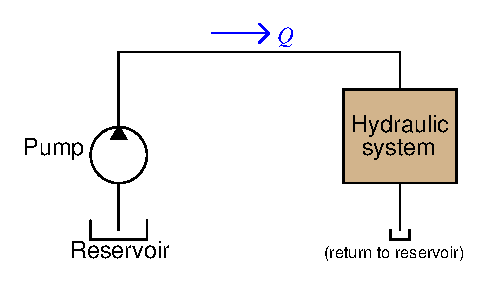
\includegraphics[width=15.5cm]{i00761x01.eps}$$

Men hvilken type elektrisk kilde etterligner best en fortrengnings-hydraulikkpumpe som roterer med konstant hastighet, en {\it spenningskilde} eller en {\it strømkilde}?

$$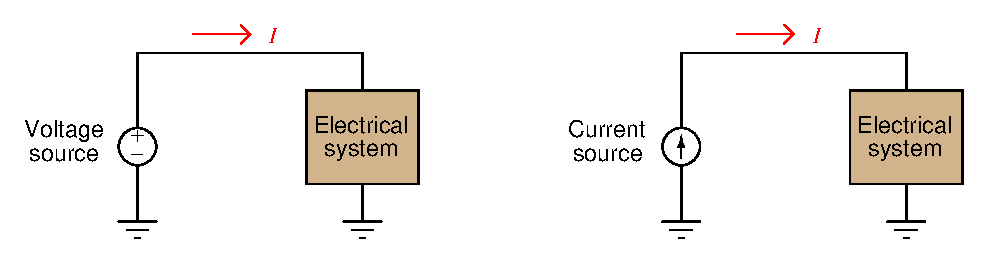
\includegraphics[width=15.5cm]{i00761x02.eps}$$

I tillegg må noe i den elektriske modellen representere luftens kompressibilitet. Hva er dette «noe annet»?

\underbar{file i00761}
%(END_QUESTION)





%(BEGIN_ANSWER)

Fortrengnings-hydraulikkpumper som går med konstant hastighet modelleres best som {\it strømkilder}, og derfor trenger de trykkavlastningsventiler for å holde hydraulikktrykket («spenningen») konstant.

%(END_ANSWER)





%(BEGIN_NOTES)

$$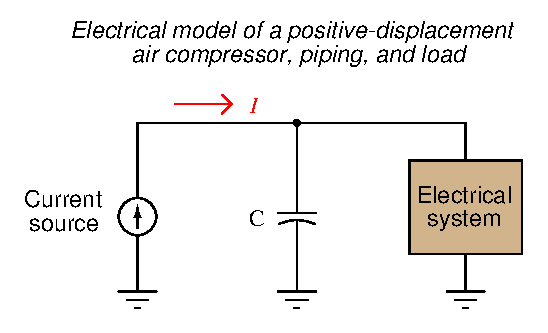
\includegraphics[width=15.5cm]{i00761x03.eps}$$

%INDEX% Mekanikk, fluidkraftsystemer: fortrengningspumpe sammenlignet med elektrisk strømkilde

%(END_NOTES)


